\section{Demonstration}

A web-based dog vocalization labeling system can intuitively show us its energy diagram and spectrogram, and we can also refer to this intuitive representation to verify whether the phonemes with the same label are the same. The system can be used to further explore the question of whether dog vocalization has certain meanings. The system is mainly divided into three parts. The first part is the introduction, which introduces how the back-end implements the dog vocalization labeling system and provides a clustering center distribution diagram of the clustering results of the model reduced to two dimensions by PCA, and how to use the other two functions.

\begin{figure*}[h]
    \centering
    \scalebox{0.4}{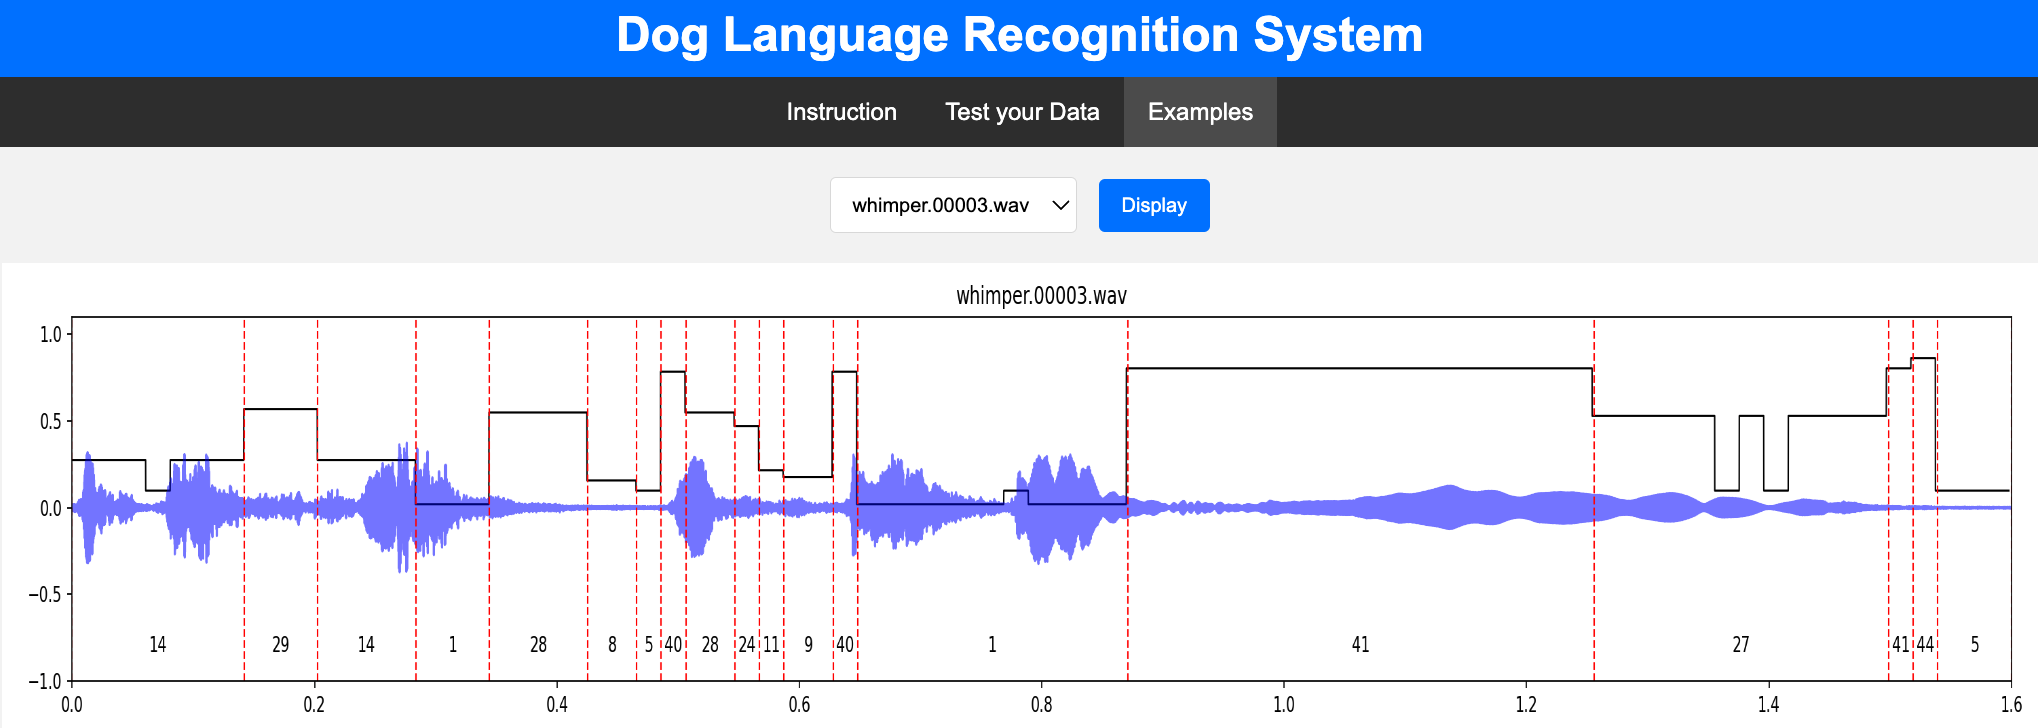
\includegraphics{demo.png}}
    \caption{Examples interface of Dog Language Recognition System.}
    \label{fig:demo1}
\end{figure*}

The second part provides users with the function of transcribing their own recorded dog vocalization, and displays their energy diagram, spectrogram, and corresponding label sequence, the interface of main page is shown as \figref{fig:demo1}. The original label sequence that has not undergone the Phone Combination operation will also be represented in the energy diagram, which can be compared with its final label and with the audio to measure the performance of the phone combination algorithm. It also supports listening to the sound of each label's corresponding phoneme alone, and the audio clip of the ``word'' in the vocabulary we found. In the next step, this page will also support the playback of video clips corresponding to the audio clips, so as to further study the meaning of each word.

The system also provides a sample display function. Each word in the vocabulary and its sound are displayed on this page, and 20 dog language sentences from the training dataset are randomly selected so that users who do not have dog vocalization samples can experience the functions of the system.